\section{XSeparation code generation in a nutshell}
\label{sec:butshell}
%In MDE, an architecture model is usually transformed into executable code through a set of transformations.
%The latter ease development of a code generator but make the traceability between the model and the code hard.
%The abstraction gap and the lack of traceability between the architecture and code, as pointed out in Section \ref{sec:intro}, make the synchronization of architecture model and code difficult.

This section presents overview of XSeparation.
For a component whose structure is described by UML components, parts, ports, and connectors and behavior by a UML State Machine, the structure- and the behavior-prescribed code are generated within the same object-oriented class. 

Fig. \ref{fig:xseparationoverview} shows the overview of the code generation in XSeparation.
A component \ttt{System} is generated to code of an object-oriented class, which consists of five code parts defined as followings:
\begin{itemize}
	\item \tb{Component structure-prescribed code:} It is generated from the component structure, which is described by UML class and component diagram structural concepts such as \ttt{property}, \ttt{port}, \ttt{part}, and \ttt{connector}.
	
	\item \tb{Behavior-prescribed code:} It is generated from the component behavior, which is described by UML State Machine diagrams and UML-defined events such as \ttt{CallEvent}, \ttt{TimeEvent}, \ttt{SignalEvent}, and \ttt{ChangeEvent}.
	
	\item \tb{State machine action code:} It is used to define fine-grained action code for the state machine actions such as state entry/exit/doActivity and transition effect.
	This code can also be generated from the model in case of industrial tools such as IBM Rhapsody and Enterprise Architect, which allow to embed the fine-grained code within the model as blocks of text.
	This code, which will be invoked by the state machine behavior of the component, has an agreement (\ttt{BP-U Agreement}) with \tb{Behavior-prescribed code}.
	The details of \ttt{BP-U Agreement} are presented in Section \ref{sec:xseparationbehavior}. 
	
	\item \tb{User-filled skeleton code:} This code contains object-oriented methods generated from UML operations defined in the model for the component.
	Similar \tb{State machine action code}, users can fill fine-grained code within the model for the operations.
	The methods can be called by \tb{State machine action code} or \tb{Component structure-provided implementation}.
	
	\item \tb{Component structure-provided implementation:} A component might provide some interfaces through its ports in order for other components to interact with. 
	This code part is for the implementation of the interfaces.
	If \tb{Architecture-prescribed code} contains a port, which provides an interface and is not delegated (connected) to an other port of one of the sub-components (see Section \ref{sec:xseparationarchitecture} for more details).  
	
\end{itemize} 

\begin{figure}
	\centering
	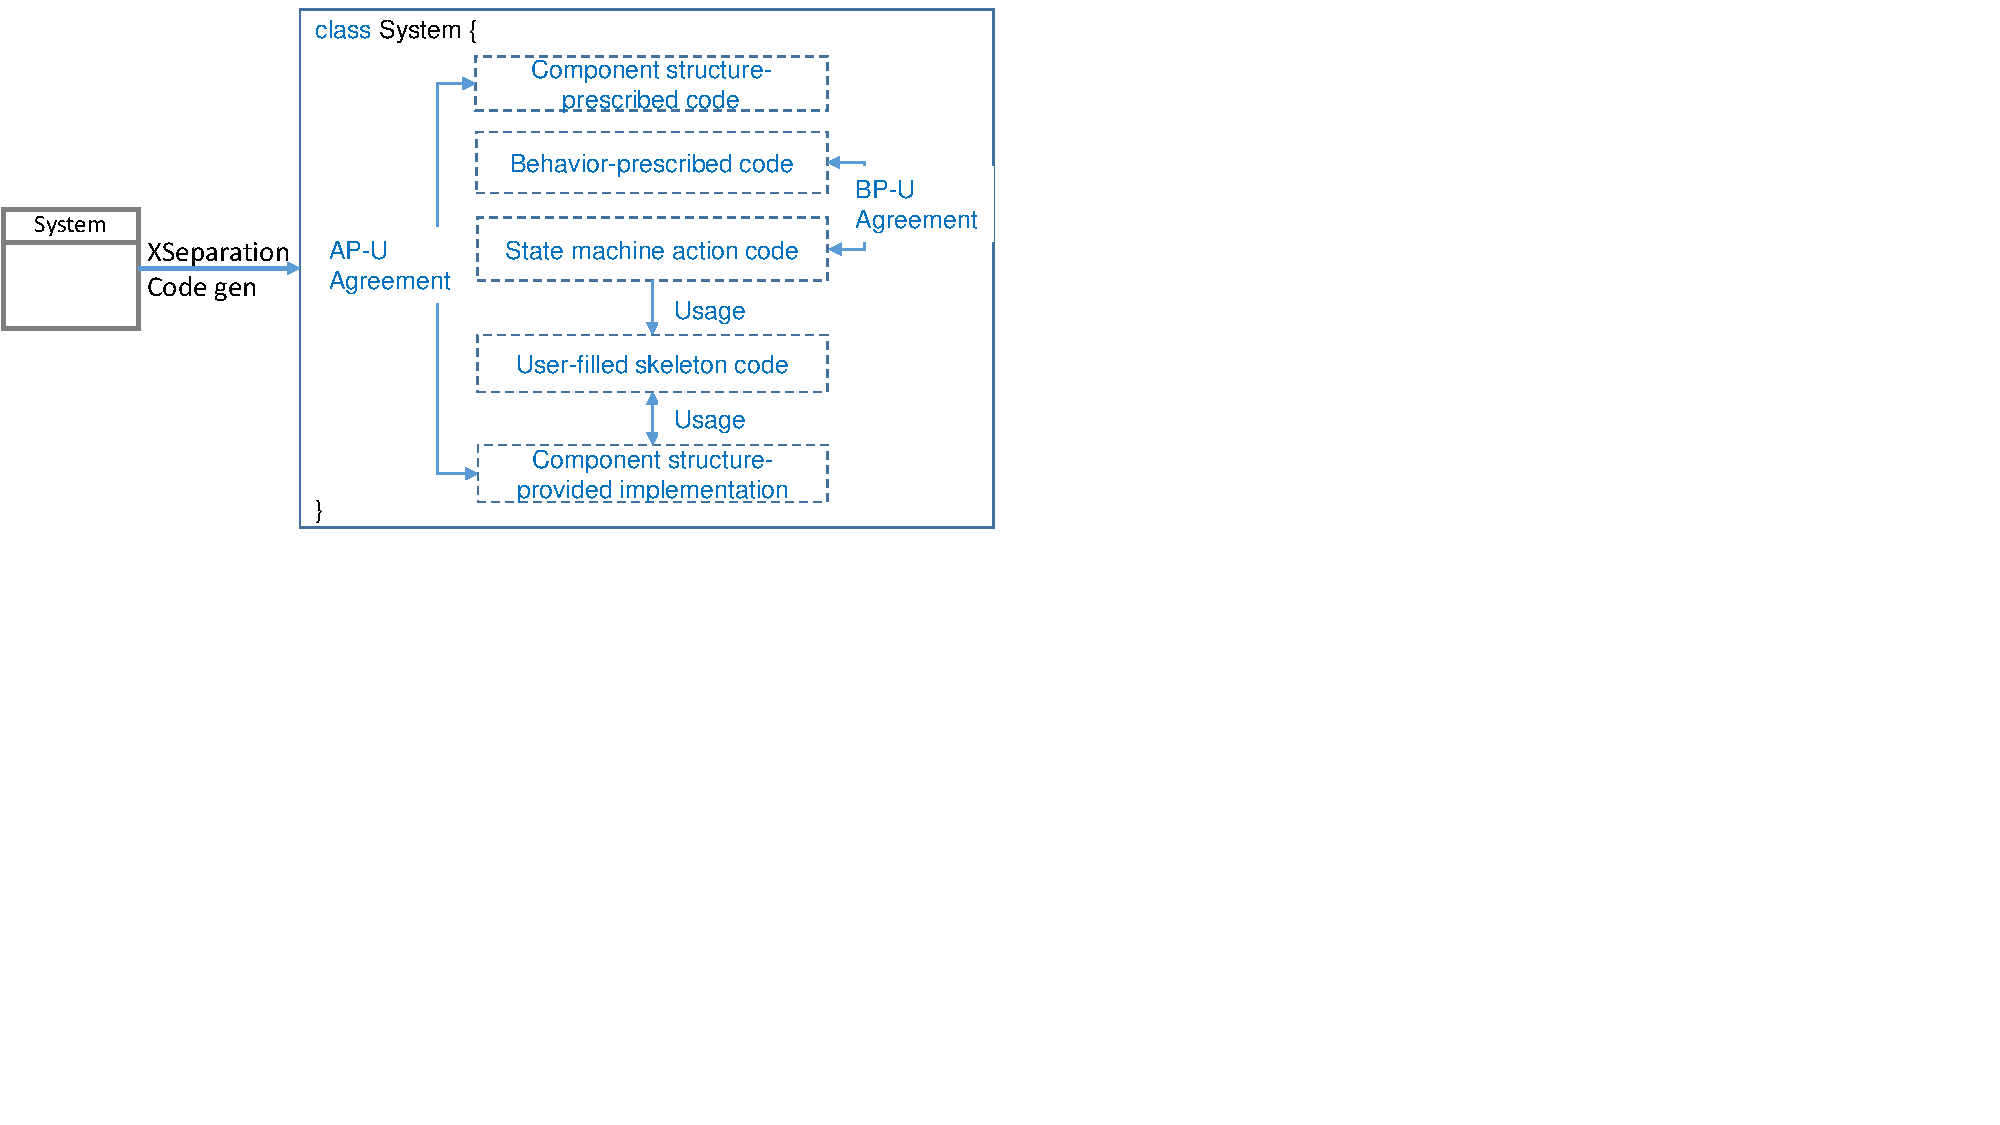
\includegraphics[clip, trim=0cm 10cm 16.8cm 0cm, width=\columnwidth]{figures/xseparationoverview.pdf}
	\caption{XSeparation overview} 
	\label{fig:xseparationoverview}
\end{figure}

Although the five parts are ideally separate from each other as in Fig. \ref{fig:xseparationoverview}, these parts, except \tb{Behavior-prescribed code}, can be populated in an interleaved way.

In the following sections, we will present the details of these parts with an illustrative example.

%\subsection{Proposed Solution}
\label{subsec:langrequirement}
\begin{itemize}
	\item The intermediate language has the ability to connect to the architecture model through a trivial mapping between the architecture and this language.
	We propose concepts closely mapped to the architecture concepts.
	
	\item A synchronization mechanism must be established between the architecture model and the intermediate language in case of concurrent synchronization. 
	We propose a synchronization mechanism.
	
	\item The intermediate language must be textual for programmers' perception, contain mechanisms and constructs to specify fine-grained statements, computational algorithms that can be done in OOPLs can be done, and must be similar to object-oriented languages so that programmers can easily use it.
	
\end{itemize}